\documentclass{article}
\usepackage[utf8]{inputenc}
\usepackage[english]{babel}

\usepackage[backend=bibtex,defernumbers=true]{biblatex}\usepackage{amsmath}
\usepackage{amssymb}
\usepackage{graphicx}
\graphicspath{ {./images/} }

\title{EEG Literature}
\author{Ravikiran Parameshwara}
\date{March 2021}
\addbibresource{literature.bib}
\begin{document}

\maketitle

\section{Introduction}
\section{Literature}
\subsection{Learning Representations from EEG with Deep Recurrent-Convolution Neural Networks (ICLR 2016) \cite{bashivan2015learning}}
Learning representations that are invariant to inter-and intra-subject differences, as well as to inherent noise associated with EEG data collection is one of the challenging tasks in modelling events from EEG data. The authors propose an approach for learning such representations. First, they transform EEG activities into a sequence of topology-preserving multi-spectral images. Next, they train RCNN to learn robust representations from the sequence of images.


\subsubsection{Making Images from EEG Time-Series}
The EEG electrodes are distributed over the scalp in a three-dimensional space. In order to transform the spatially distributed activity maps as 2-D images, we need to first project the location of electrodes from a 3-dimensional space onto a 2-D surface. However, such transformation should also preserve the relative distance between neighboring electrodes. For this purpose, authors used the Azimuthal Equidistant Projection (AEP) also known as Polar Projection, borrowed from mapping applications. Width and height of the image represent the spatial distribution of activities over the cortex. We apply Clough- Tocher scheme for interpolating the scattered power measurements over the scalp and for estimating the values in-between the electrodes over a $32\times32$ mesh. This procedure is repeated for each frequency band of interest, resulting in three topographical activity maps corresponding to each frequency band. The three spatial maps are then merged together to form an image with three (color) channels.


\begin{figure}[h]
    \centering
    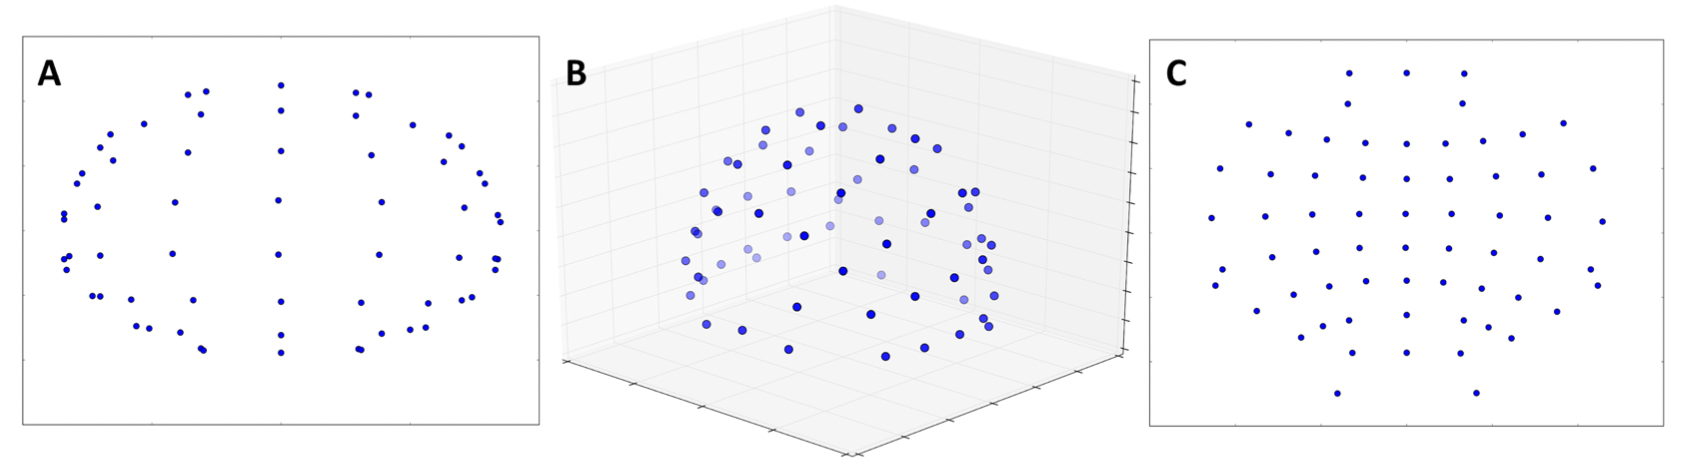
\includegraphics[width=\textwidth]{azim_proj_eeg.png}
    \caption{Topology-preserving and non-topology-preserving projections of electrode locations. A) 2-D projection of electrode locations using non-topology-preserving simple orthographic projection. B) Location of electrodes in the original 3-D space. C) 2-D projection of electrode locations using topology-preserving azimuthal equidistant projection.}
    \label{fig:azim_proj_eeg}
\end{figure}


\subsection{Architecture}

\printbibliography

%\medskip

%\bibliographystyle{unsrt}
%\bibliography{literature.bib}
\end{document}
